\documentclass[11pt]{beamer}
\usetheme{Luebeck}
\usepackage[utf8]{inputenc}
\usepackage[english]{babel}
\usepackage{amsmath}
\usepackage{siunitx}
\usepackage{amsfonts}
\usepackage{amssymb}
\usepackage{graphicx}
\usepackage{booktabs}
\usepackage{subcaption}
\usepackage[compat=1.0.0]{tikz-feynman}
\tikzfeynmanset{
  my dot/.style={
    /tikzfeynman/dot,
    /tikz/minimum size=3pt,
  },
}

\author{Eugenia Spedicato, Lina Maria Ortiz Parra, Jonah Blank}
\title{Detector induced assymetry in CP violation measurements}
%\setbeamercovered{transparent}
%\setbeamertemplate{navigation symbols}{}
%\logo{}
%\institute{}
%\date{}
%\subject{}
\begin{document}

\begin{frame}
\titlepage
\end{frame}

\begin{frame}
\tableofcontents
\end{frame}
\section*{Efficiency measurements in GEN-level MC}
\begin{frame}{MC truth information}
\[
D^* \rightarrow D_0(K\pi)\pi
\]
\begin{itemize}
\item using MC samples \texttt{minisample\char`_Dst2D0pi\char`_D02Kpi\char`_2016\char`_Up\char`_GEN},\\
\texttt{minisample\char`_Dst2D0pi\char`_D02Kpi\char`_2016\char`_Dw\char`_GEN} for different magnet polarities
\item comparing truth level to detector simulation\\
$\rightarrow$ final state detector efficiency
\end{itemize}
\end{frame}
\begin{frame}{Efficiencies: Total, + and -}
\begin{table}
\caption{Total reconstruction efficiencies}
\resizebox{\textwidth}{!}{
	\begin{tabular}{cS[table-format=2.2]@{${}\pm{}$}S[table-format=1.2]S[table-format=2.2]@{${}\pm{}$}S[table-format=1.2]S[table-format=2.2]@{${}\pm{}$}S[table-format=1.2]S[table-format=2.2]@{${}\pm{}$}S[table-format=1.2]S[table-format=2.2]@{${}\pm{}$}S[table-format=1.2]}
		\toprule
		{Polarity} & \multicolumn{2}{c}{$\epsilon_{\pi} $} & \multicolumn{2}{c}{$\epsilon_{K} $} & \multicolumn{2}{c}{$ \epsilon_{\pi,s} $} & \multicolumn{2}{c}{$\epsilon_{D^0} $} & \multicolumn{2}{c}{$\epsilon_{D^*} $} \\
		\midrule
		$UP$ & 86.65 & 0.01 & 84.63 & 0.01 & 76.65 & 0.02 & 73.34 & 0.02 & 56.31 & 0.02\\
		$DOWN$ & 86.68 & 0.01 & 84.67 & 0.01 & 76.66 & 0.02 & 73.39 & 0.02 & 56.35 & 0.02\\
		\bottomrule
	\end{tabular}}
\caption{$D^{*+}$ reconstruction efficiencies}
\resizebox{\textwidth}{!}{
	\begin{tabular}{cS[table-format=2.2]@{${}\pm{}$}S[table-format=1.2]S[table-format=2.2]@{${}\pm{}$}S[table-format=1.2]S[table-format=2.2]@{${}\pm{}$}S[table-format=1.2]S[table-format=2.2]@{${}\pm{}$}S[table-format=1.2]S[table-format=2.2]@{${}\pm{}$}S[table-format=1.2]}
		\toprule
		{Polarity} & \multicolumn{2}{c}{$\epsilon_{\pi^+} $} & \multicolumn{2}{c}{$\epsilon_{K^-} $} & \multicolumn{2}{c}{$ \epsilon_{\pi^+,s} $} & \multicolumn{2}{c}{$\epsilon_{D_0} $} & \multicolumn{2}{c}{$\epsilon_{D^{*+}} $} \\
		\midrule
		$UP$ & 86.66 & 0.02 & 85.02 & 0.02 & 76.37 & 0.02 & 73.01 & 0.03 & 55.86 & 0.03 \\
		$DOWN$ & 86.70 & 0.02 & 85.07 & 0.02 & 76.98 & 0.02 & 73.06 & 0.03 & 56.33 & 0.03 \\
		\bottomrule
	\end{tabular}}
\caption{$D^{*-}$ reconstruction efficiencies}
\resizebox{\textwidth}{!}{
	\begin{tabular}{cS[table-format=2.2]@{${}\pm{}$}S[table-format=1.2]S[table-format=2.2]@{${}\pm{}$}S[table-format=1.2]S[table-format=2.2]@{${}\pm{}$}S[table-format=1.2]S[table-format=2.2]@{${}\pm{}$}S[table-format=1.2]S[table-format=2.2]@{${}\pm{}$}S[table-format=1.2]}
		\toprule
		{Polarity} & \multicolumn{2}{c}{$\epsilon_{\pi^-} $} & \multicolumn{2}{c}{$\epsilon_{K^+} $} & \multicolumn{2}{c}{$ \epsilon_{\pi^-,s} $} & \multicolumn{2}{c}{$\epsilon_{\bar{D}_0} $} & \multicolumn{2}{c}{$\epsilon_{D^{*-}} $} \\
		\midrule
		$UP$ & 86.65 & 0.02 & 84.25 & 0.02 & 76.93 & 0.02 & 73.67 & 0.03 & 56.76 & 0.03 \\
		$DOWN$ & 86.66 & 0.02 & 84.27 & 0.02 & 76.34 & 0.02 & 73.72 & 0.03 & 56.36 & 0.02 \\
		\bottomrule
	\end{tabular}}
\end{table}
\end{frame}
%\begin{frame}{Efficiencies}
%\begin{itemize}
%\item $A_{CP}$ is much smaller in for the $UP$-polarity
%\item in MC: $\epsilon_{D^*}=\epsilon_{\pi,s}\cdot\epsilon_{D^0}$
%\item structure of $\epsilon(\phi)$ probably due to rectangular detector shape
%\item peak in $\epsilon_{D^*}(\theta)$ within scope of error
%\end{itemize}
%\end{frame}
\begin{frame}{Asymmetry}
\begin{table}
	\caption{The asymmetry $\frac{N_+ - N_-}{N_+ + N_-}/10^{-3}$}
	\resizebox{\textwidth}{!}{
	\begin{tabular}{cS[table-format=1.1]@{${}\pm{}$}S[table-format=1.1]S[table-format=1.1]@{${}\pm{}$}S[table-format=1.1]S[table-format=1.1]@{${}\pm{}$}S[table-format=1.1]S[table-format=1.1]@{${}\pm{}$}S[table-format=1.1]S[table-format=1.1]@{${}\pm{}$}S[table-format=1.1]}
		\toprule
		{Polarity} & \multicolumn{2}{c}{$\pi $} & \multicolumn{2}{c}{$ K $} & \multicolumn{2}{c}{$ soft \pi $} & \multicolumn{2}{c}{$ D^0 $} & \multicolumn{2}{c}{$ D^* $} \\
		\midrule
		$UP$ & -0.1 & 0.4 & 4.7 & 0.4 & -3.8 & 0.5 & -4.7 & 0.5 & -8.2 & 0.5 \\
		$DOWN$ & -0.3 & 0.4 & 5.2 & 0.4 & 3.7 & 0.5 & -5.0 & 0.5 & -0.8 & 0.5\\
		\bottomrule
	\end{tabular}}
\end{table}
\begin{itemize}
\item $D_{soft\,\pi} \& D_{D^0}$ cancel partially in $DOWN$,\\
but add up in $UP$
\item $|A_{CP,D^*}|$ much bigger for the $UP$-polarity
\end{itemize}
\end{frame}
\begin{frame}{Comparison of different charges with $UP$ polarity - $D^*$}
\begin{figure}
\begin{subfigure}{0.45\textwidth}
\includegraphics[width=0.9\textwidth]{up_pdf/combined/h_pt_reco_Dst.pdf}
\end{subfigure}
\begin{subfigure}{0.45\textwidth}
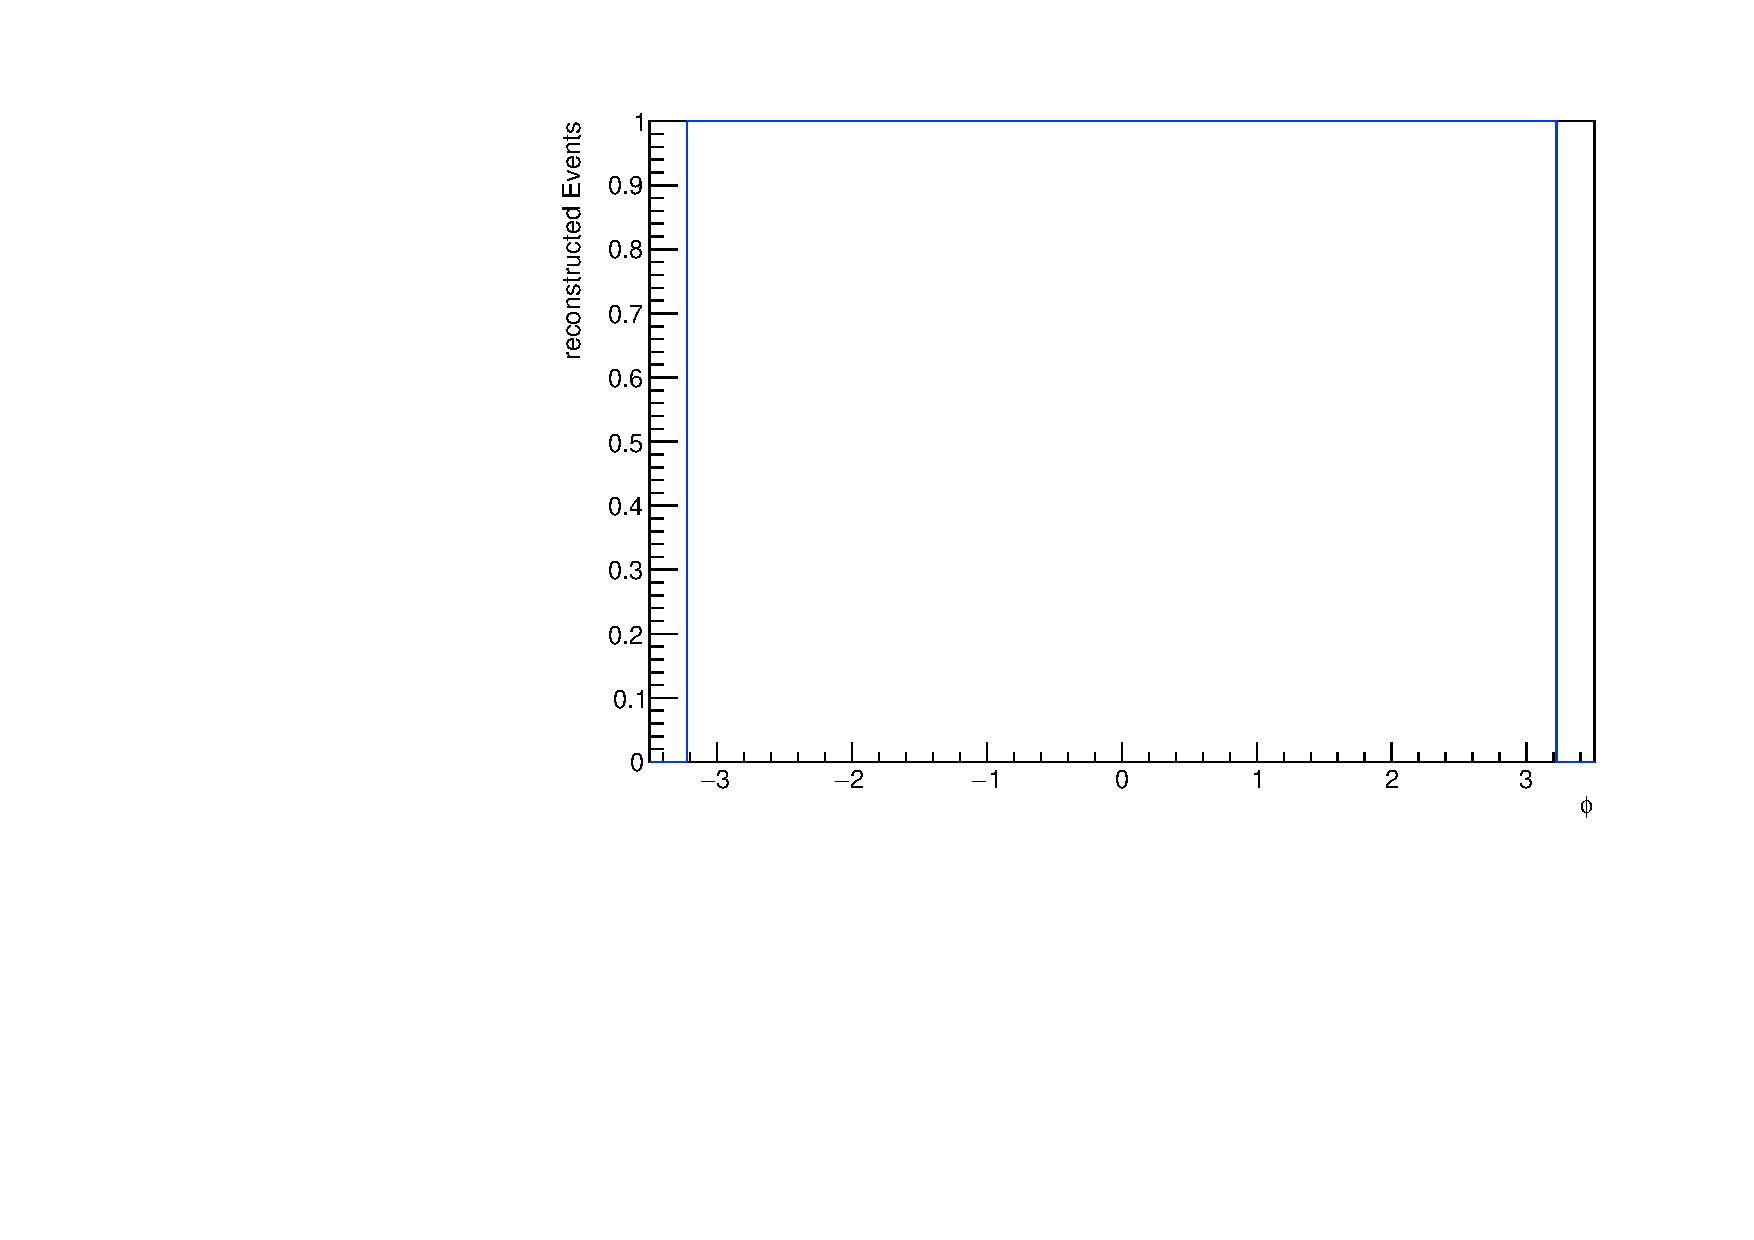
\includegraphics[width=0.9\textwidth]{up_pdf/combined/h_phi_reco_Dst.pdf}
\end{subfigure}
\begin{subfigure}{0.45\textwidth}
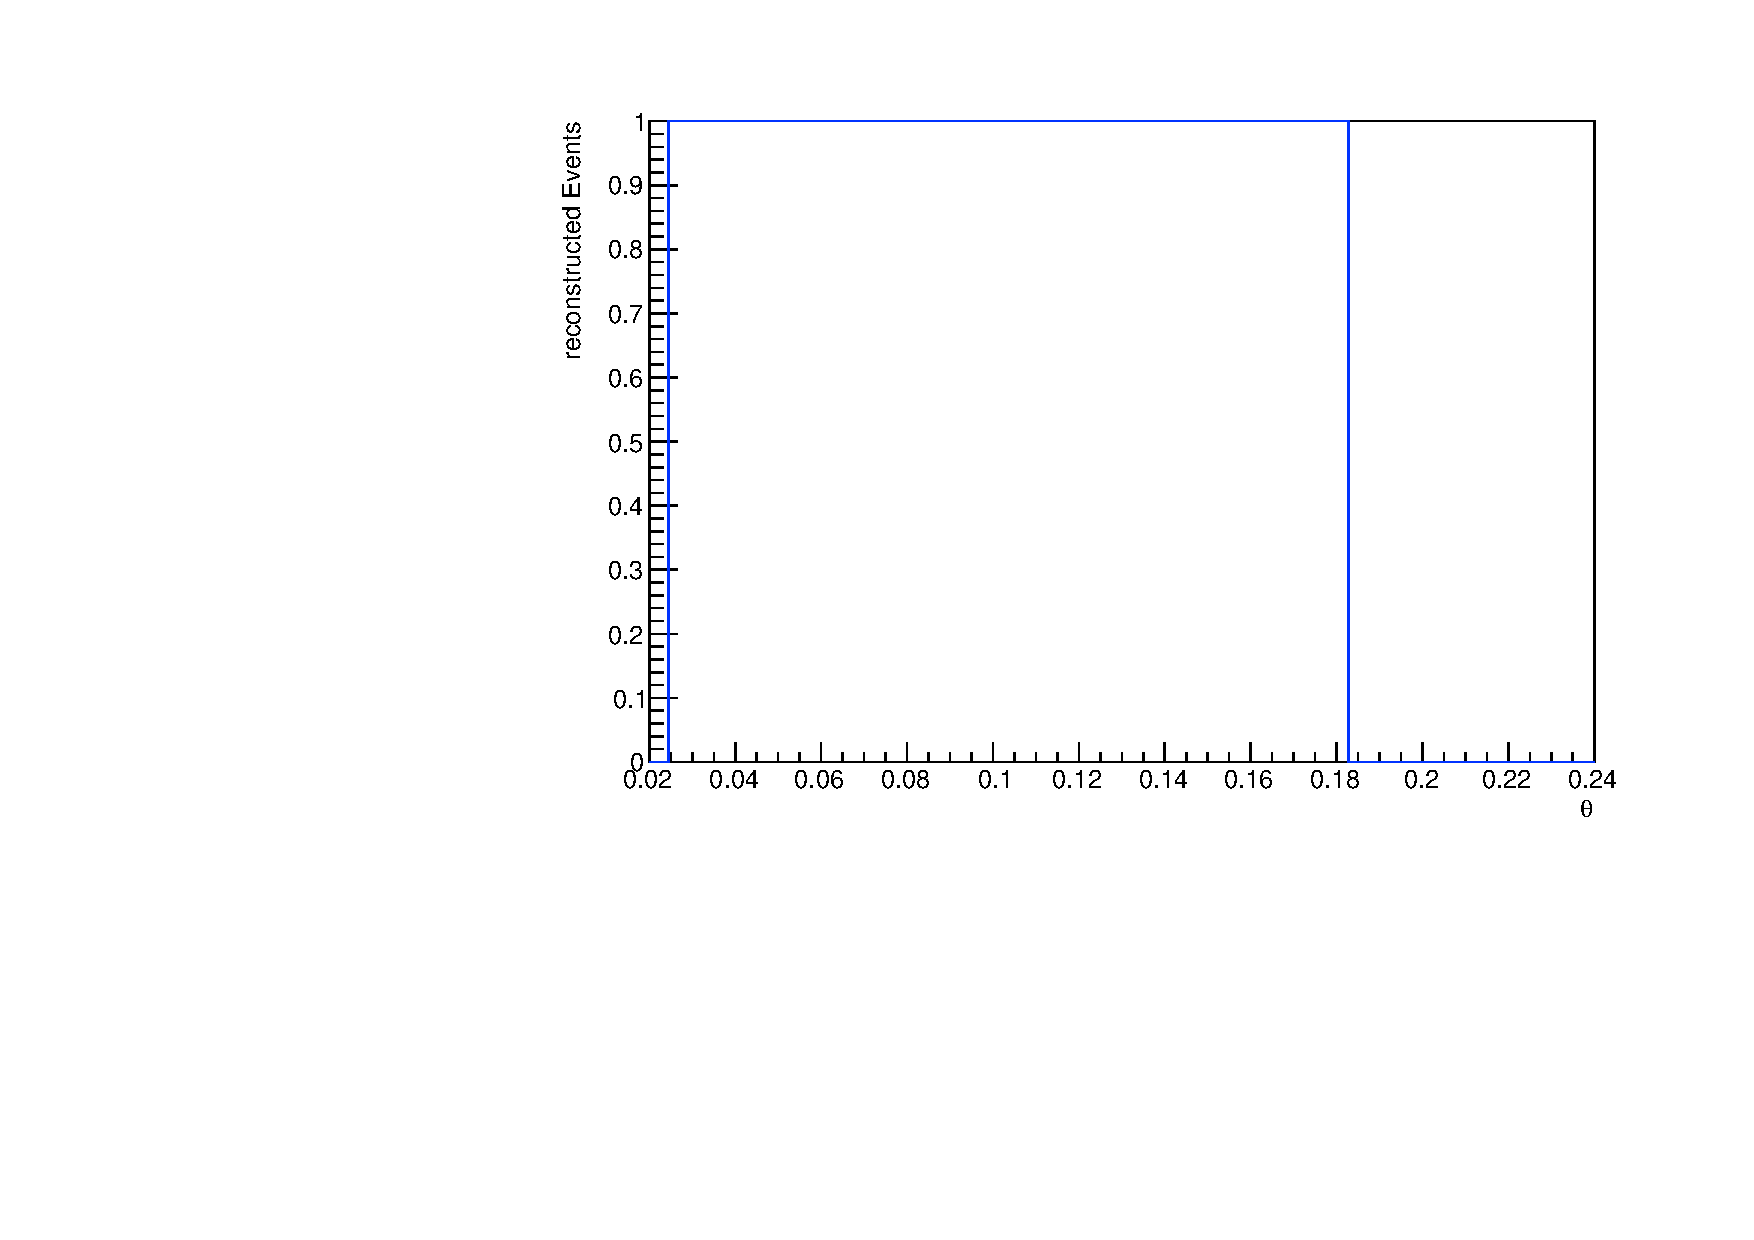
\includegraphics[width=0.9\textwidth]{up_pdf/combined/h_theta_reco_Dst.pdf}
\end{subfigure}
\begin{subfigure}{0.45\textwidth}
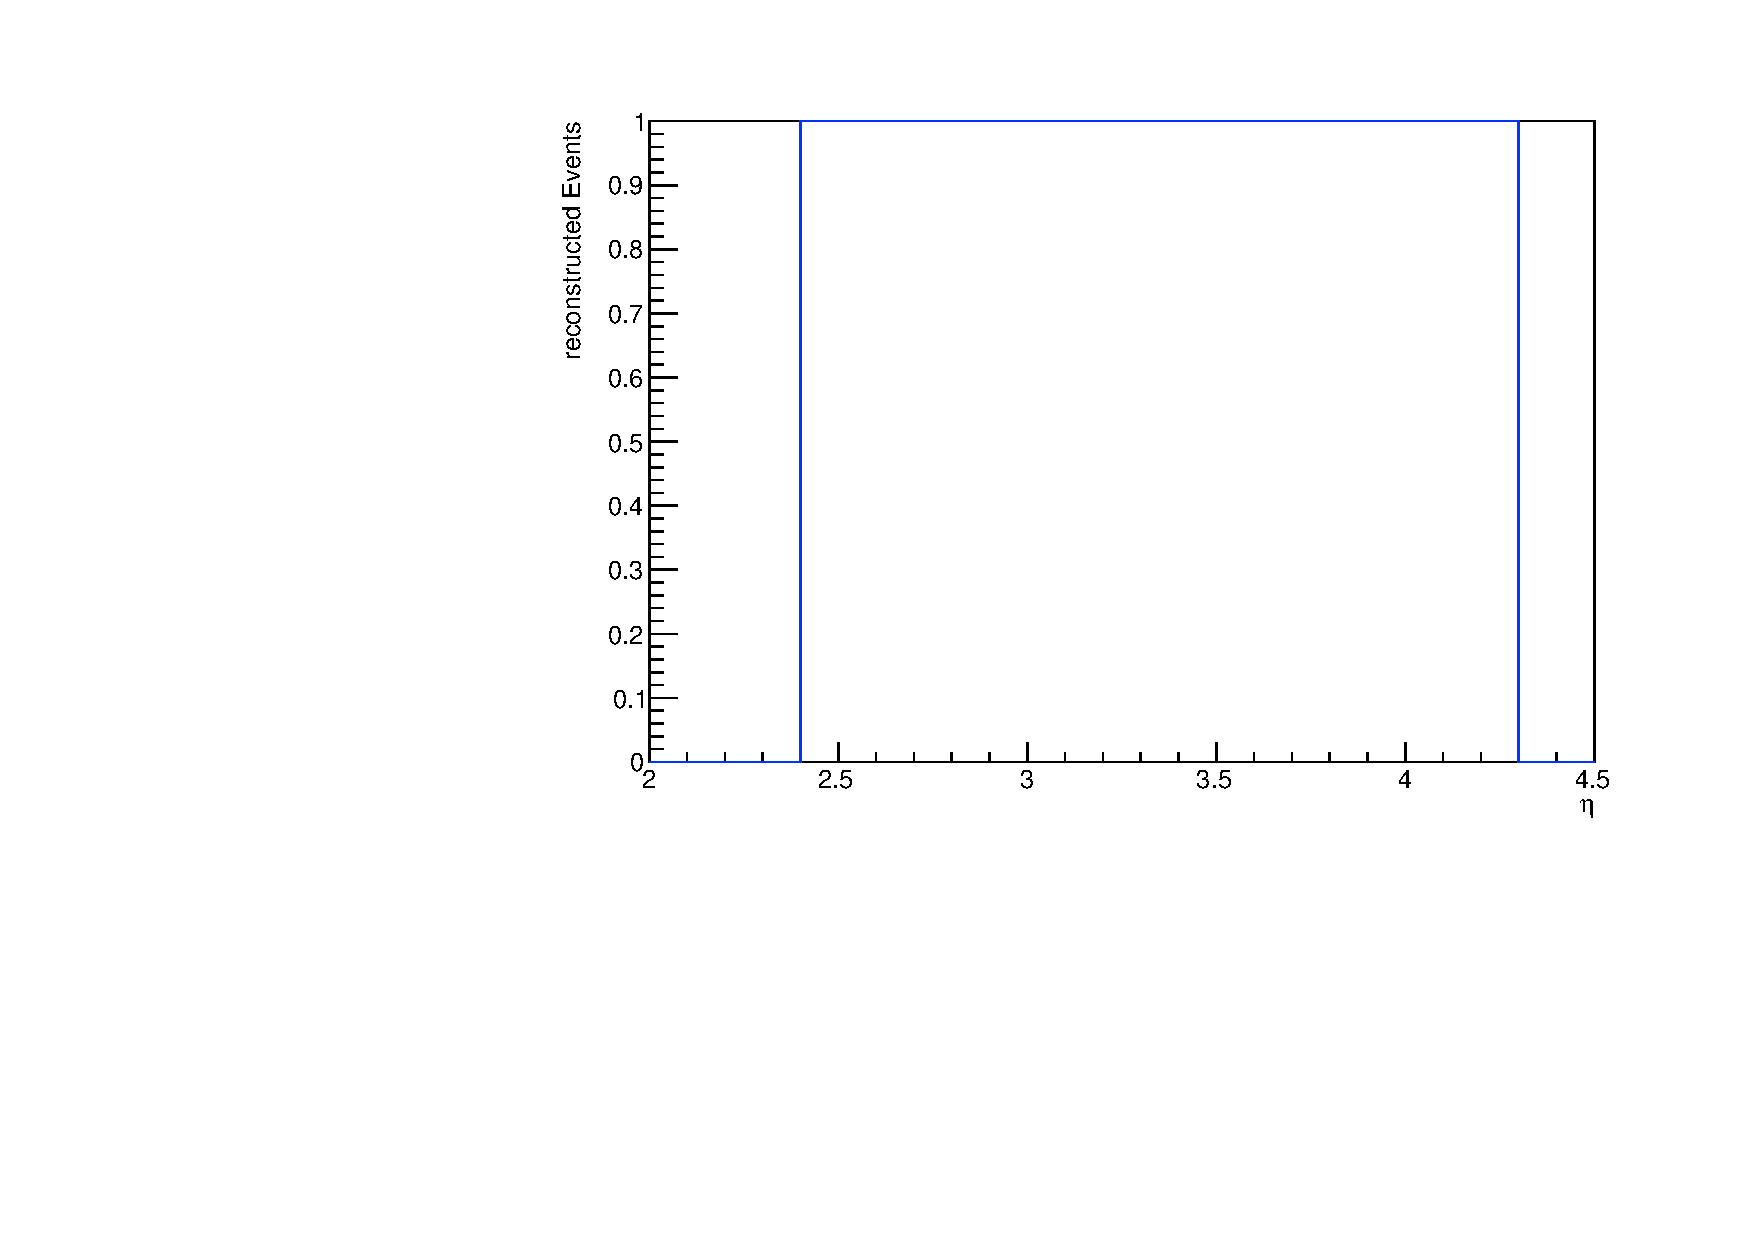
\includegraphics[width=0.9\textwidth]{up_pdf/combined/h_eta_reco_Dst.pdf}
\end{subfigure}
\end{figure}
\end{frame}
\begin{frame}{Comparison - $D^* \phi$}
\centering
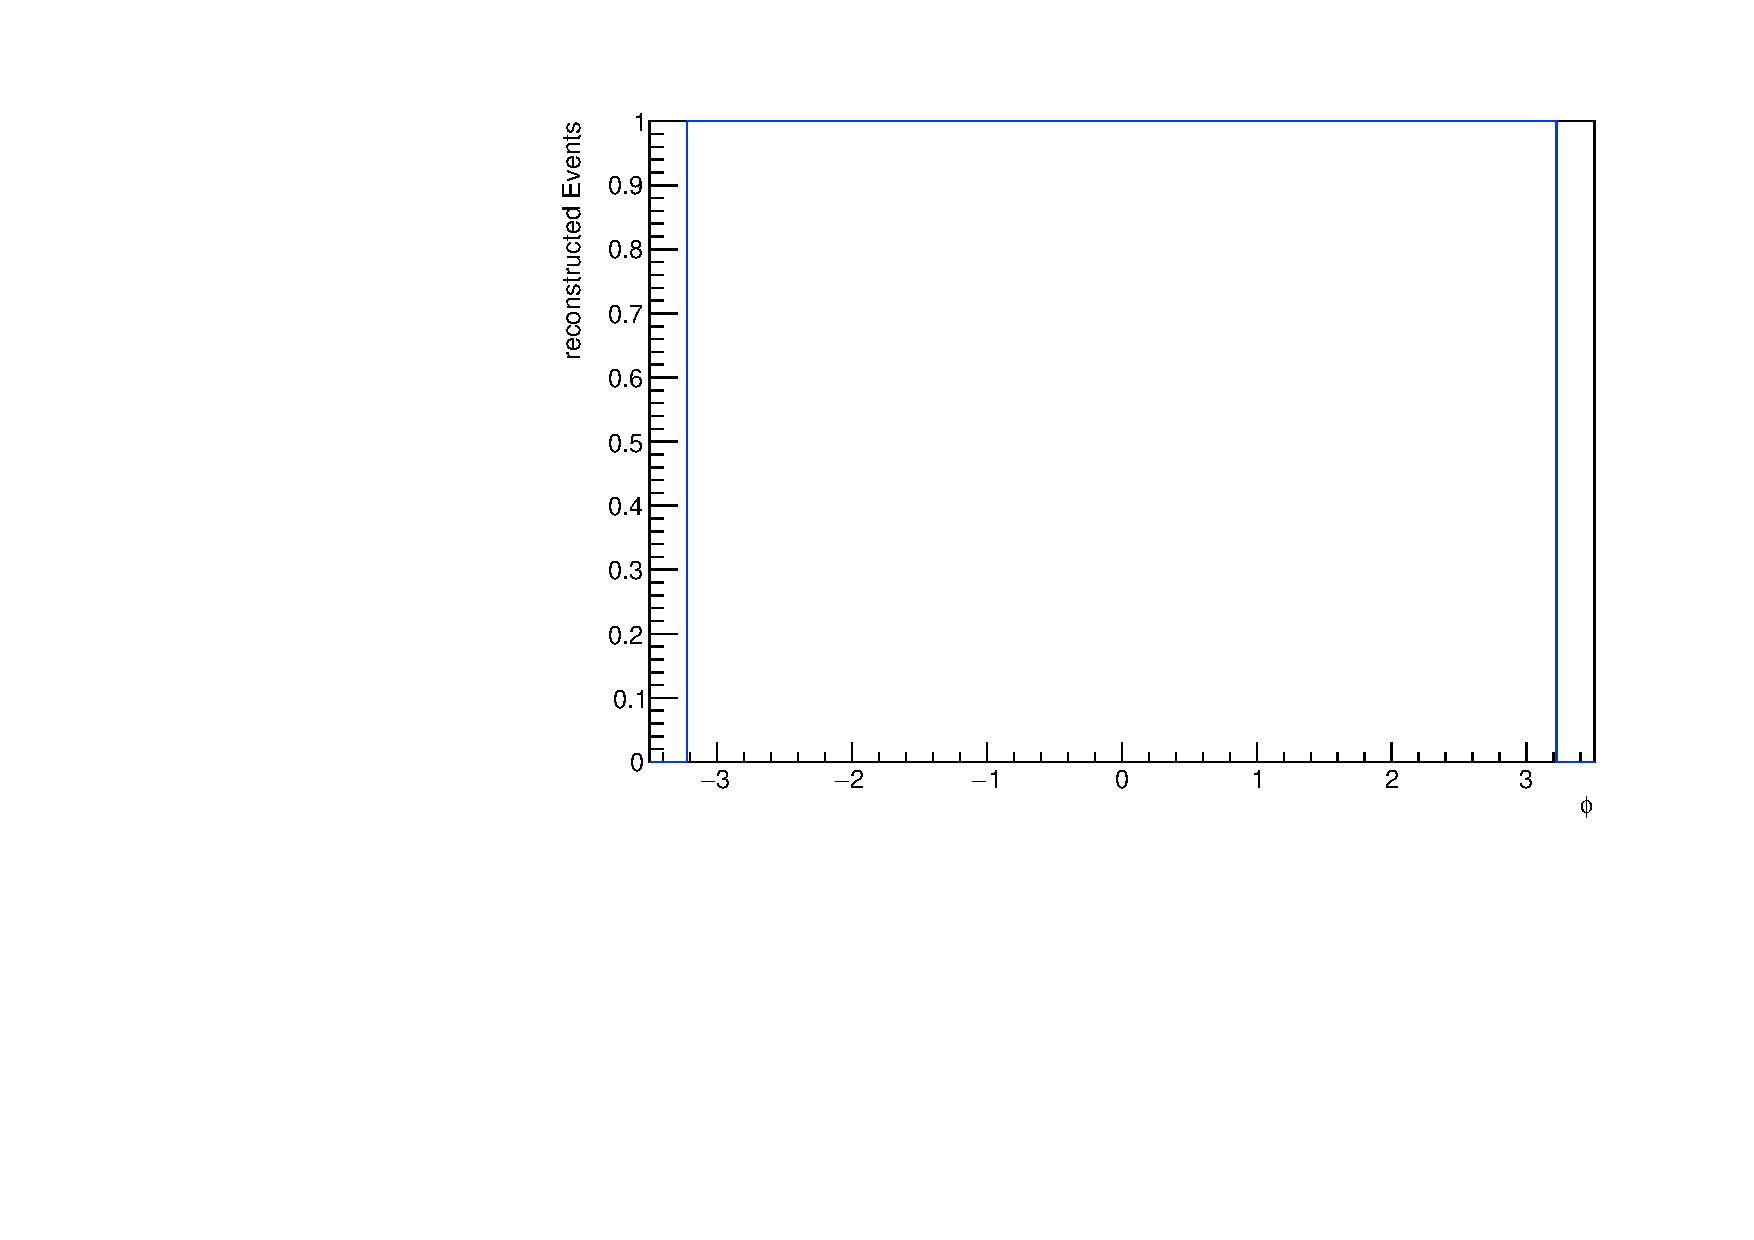
\includegraphics[width=0.48\textwidth]{up_pdf/combined/h_phi_reco_Dst.pdf}
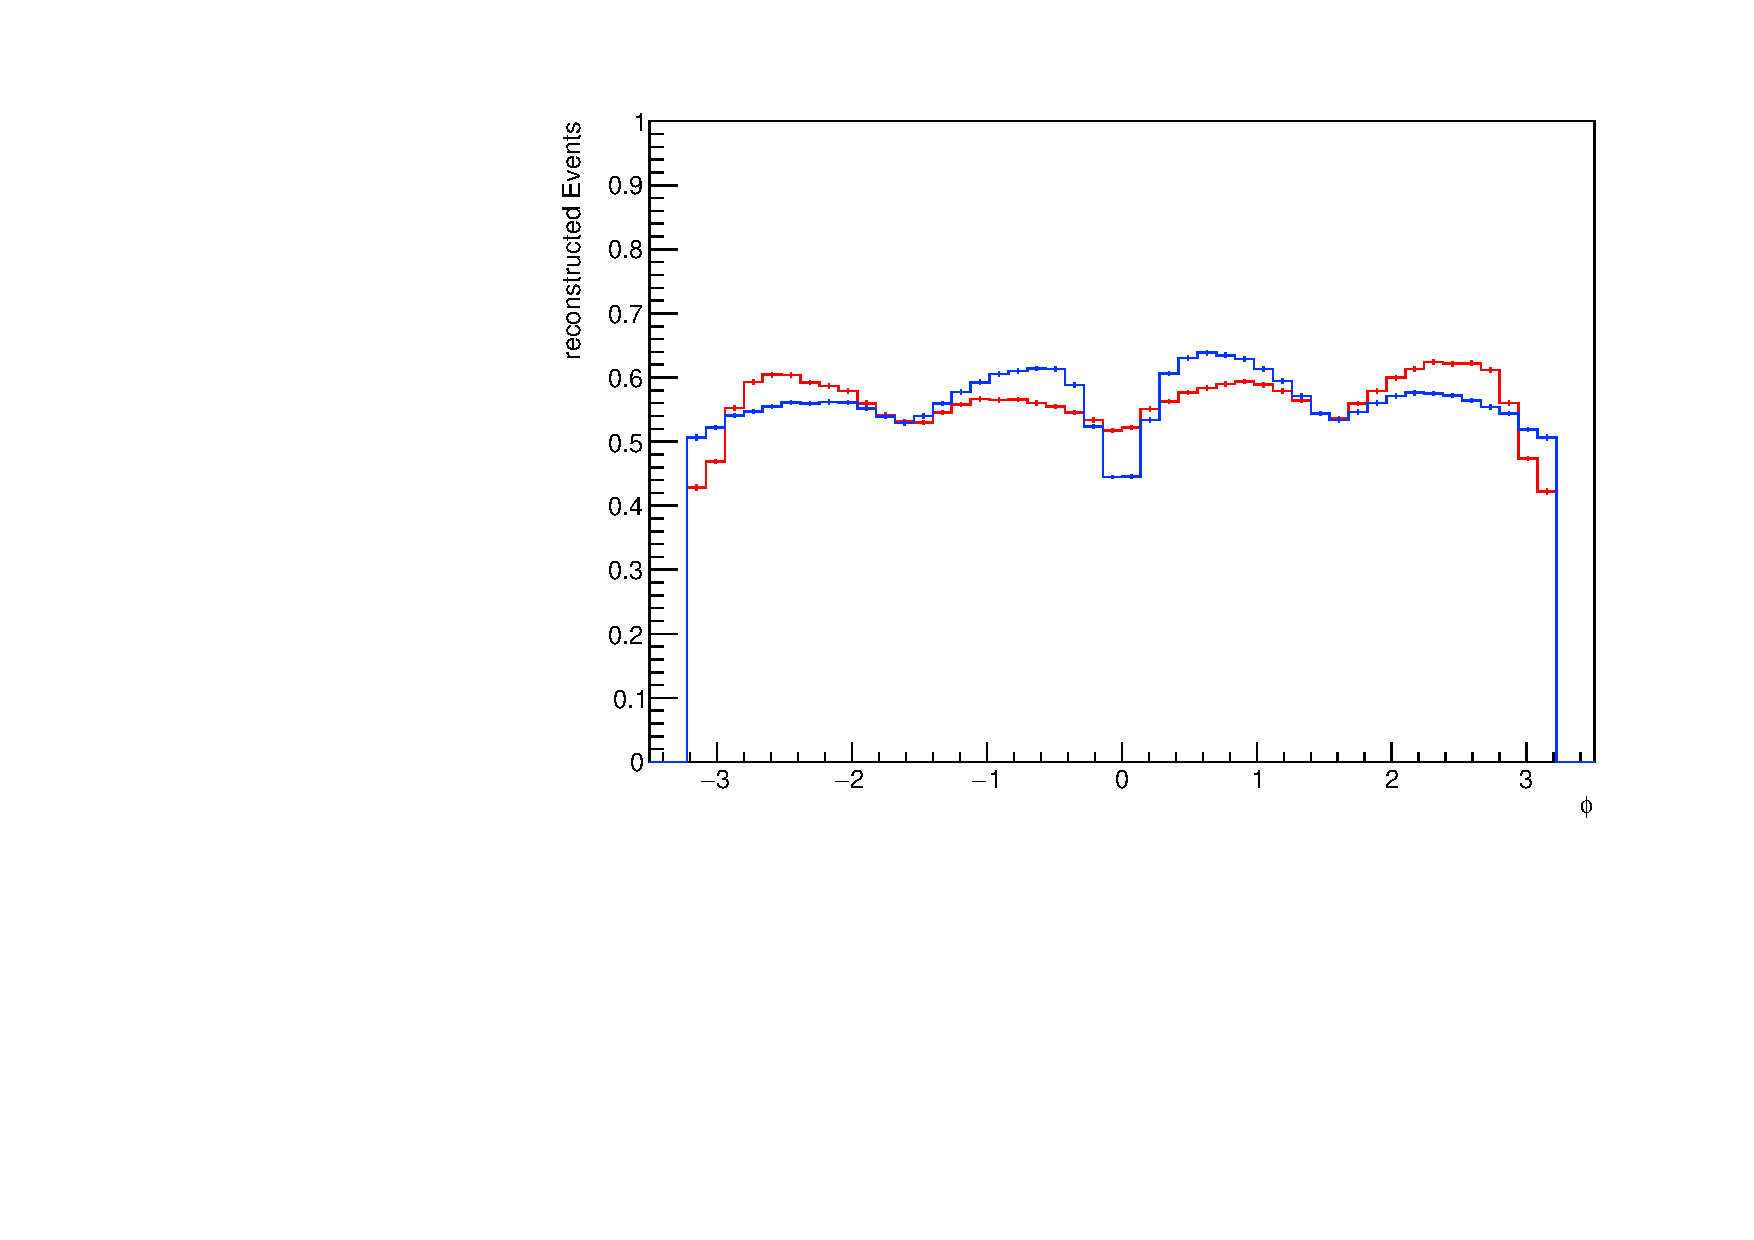
\includegraphics[width=0.48\textwidth]{down_pdf/combined/h_phi_reco_Dst.pdf}
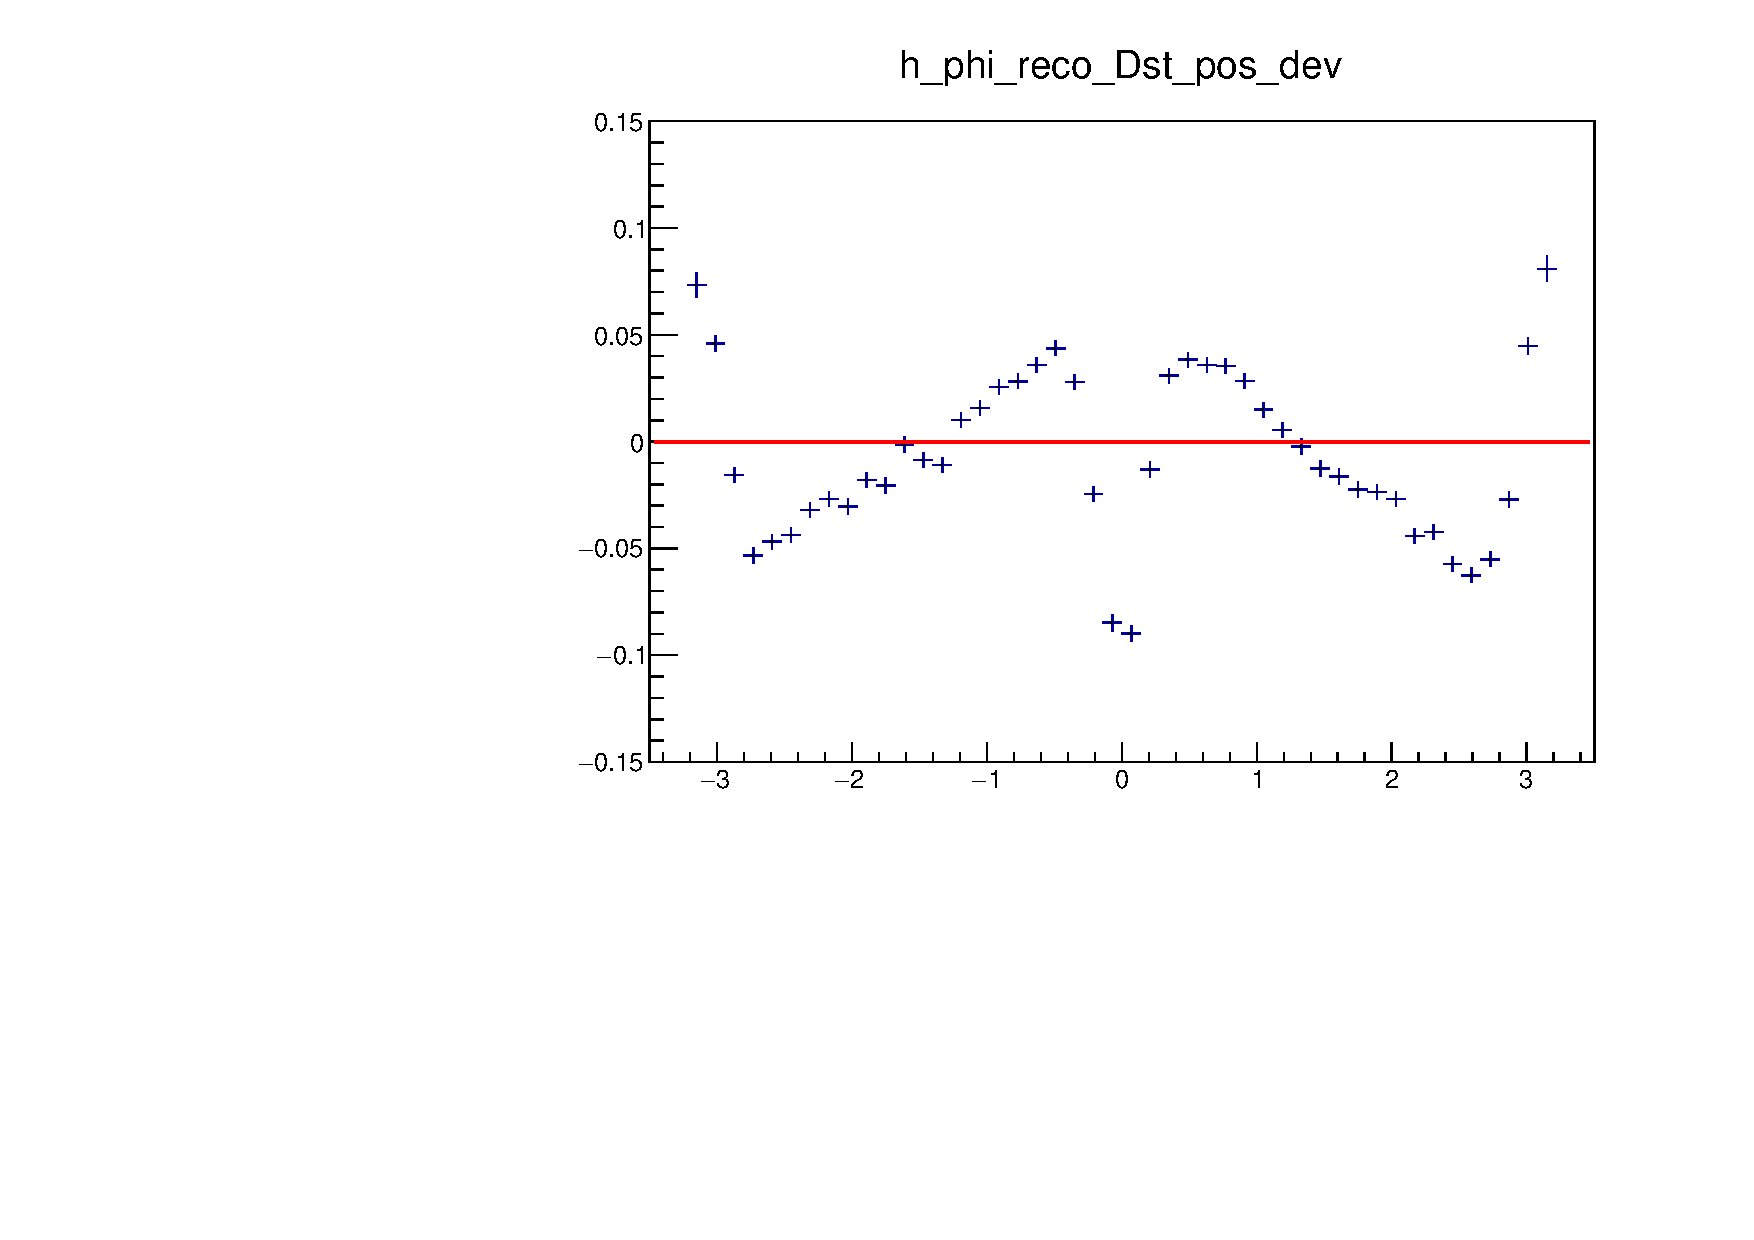
\includegraphics[width=0.48\textwidth]{up_pdf/deviation/h_phi_reco_Dst_pos_dev.pdf}
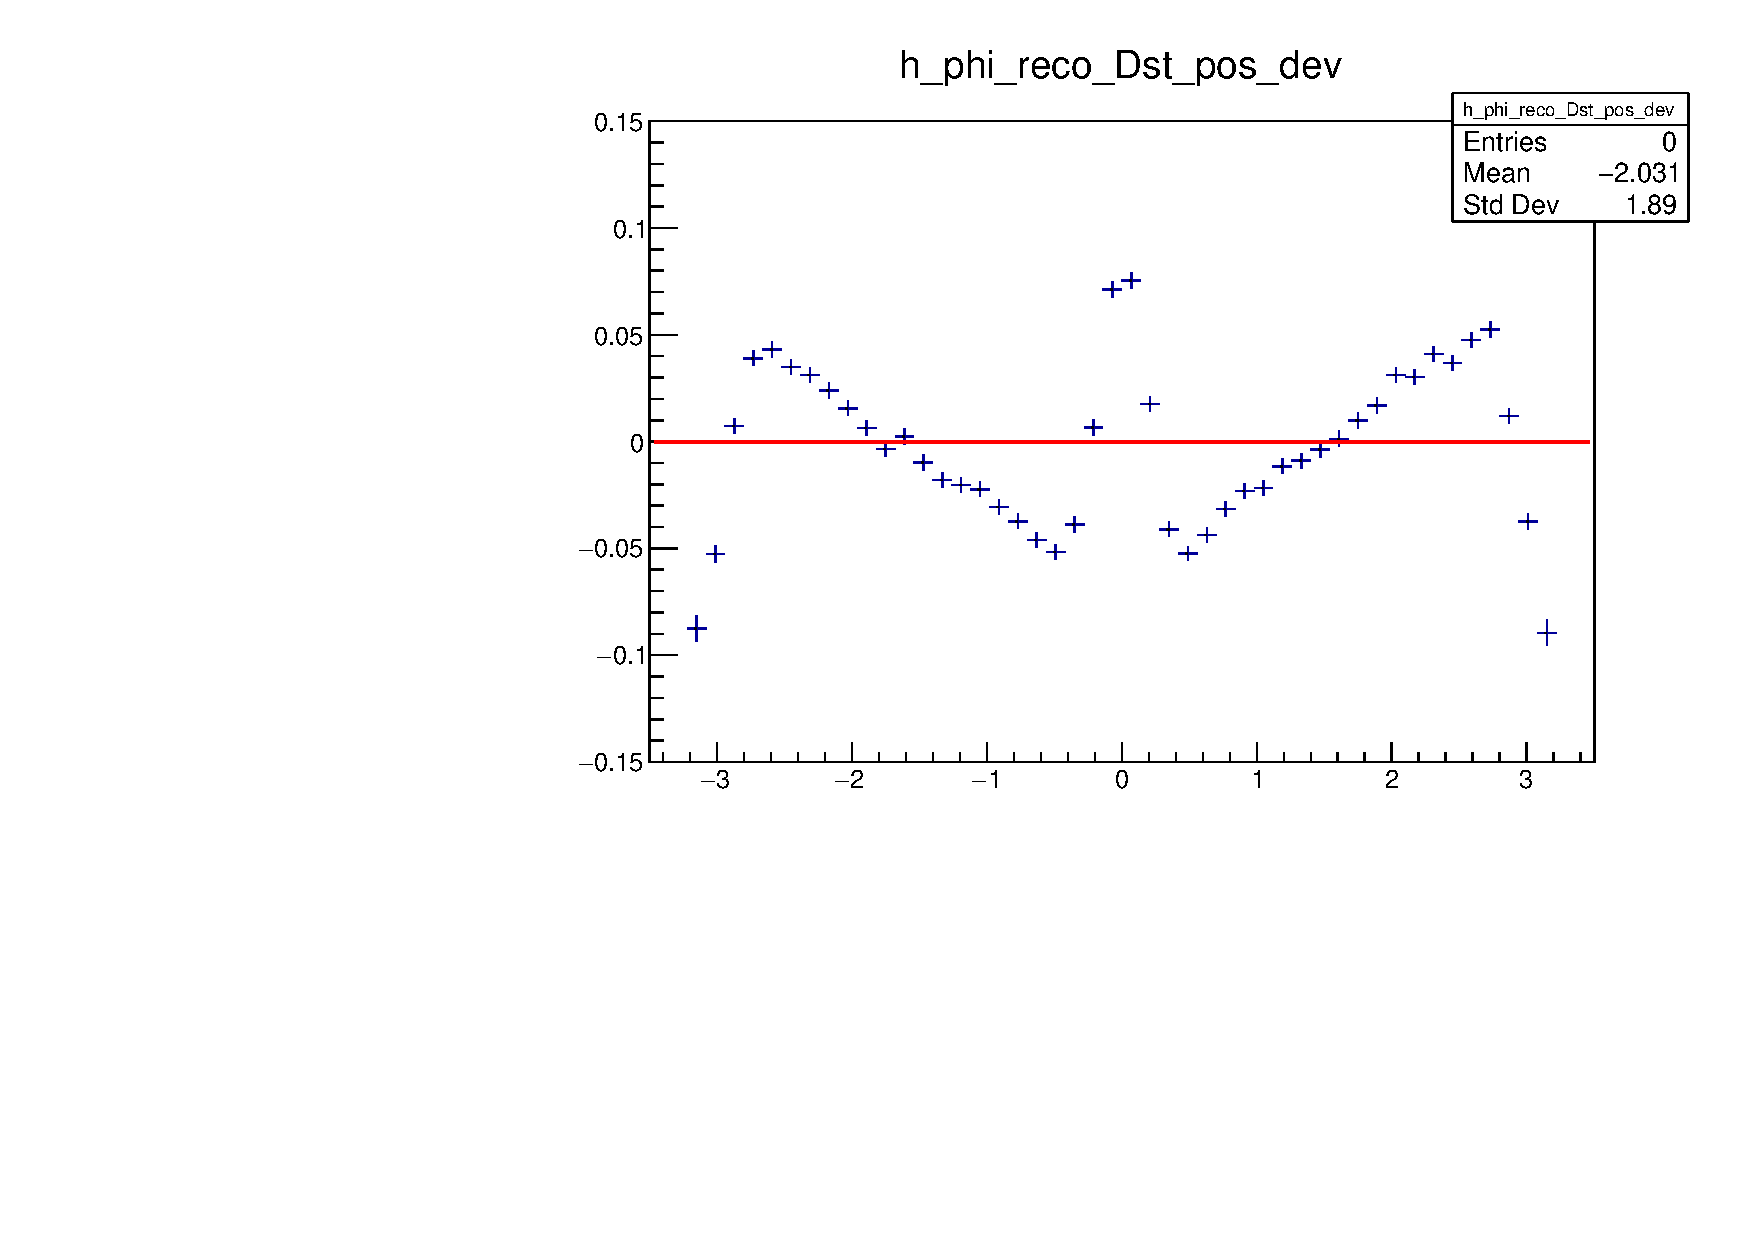
\includegraphics[width=0.48\textwidth]{down_pdf/deviation/h_phi_reco_Dst_pos_dev.pdf}
\end{frame}
\begin{frame}{$D^*$ asymmetry UP+DOWN}
\begin{figure}
\begin{subfigure}{0.45\textwidth}
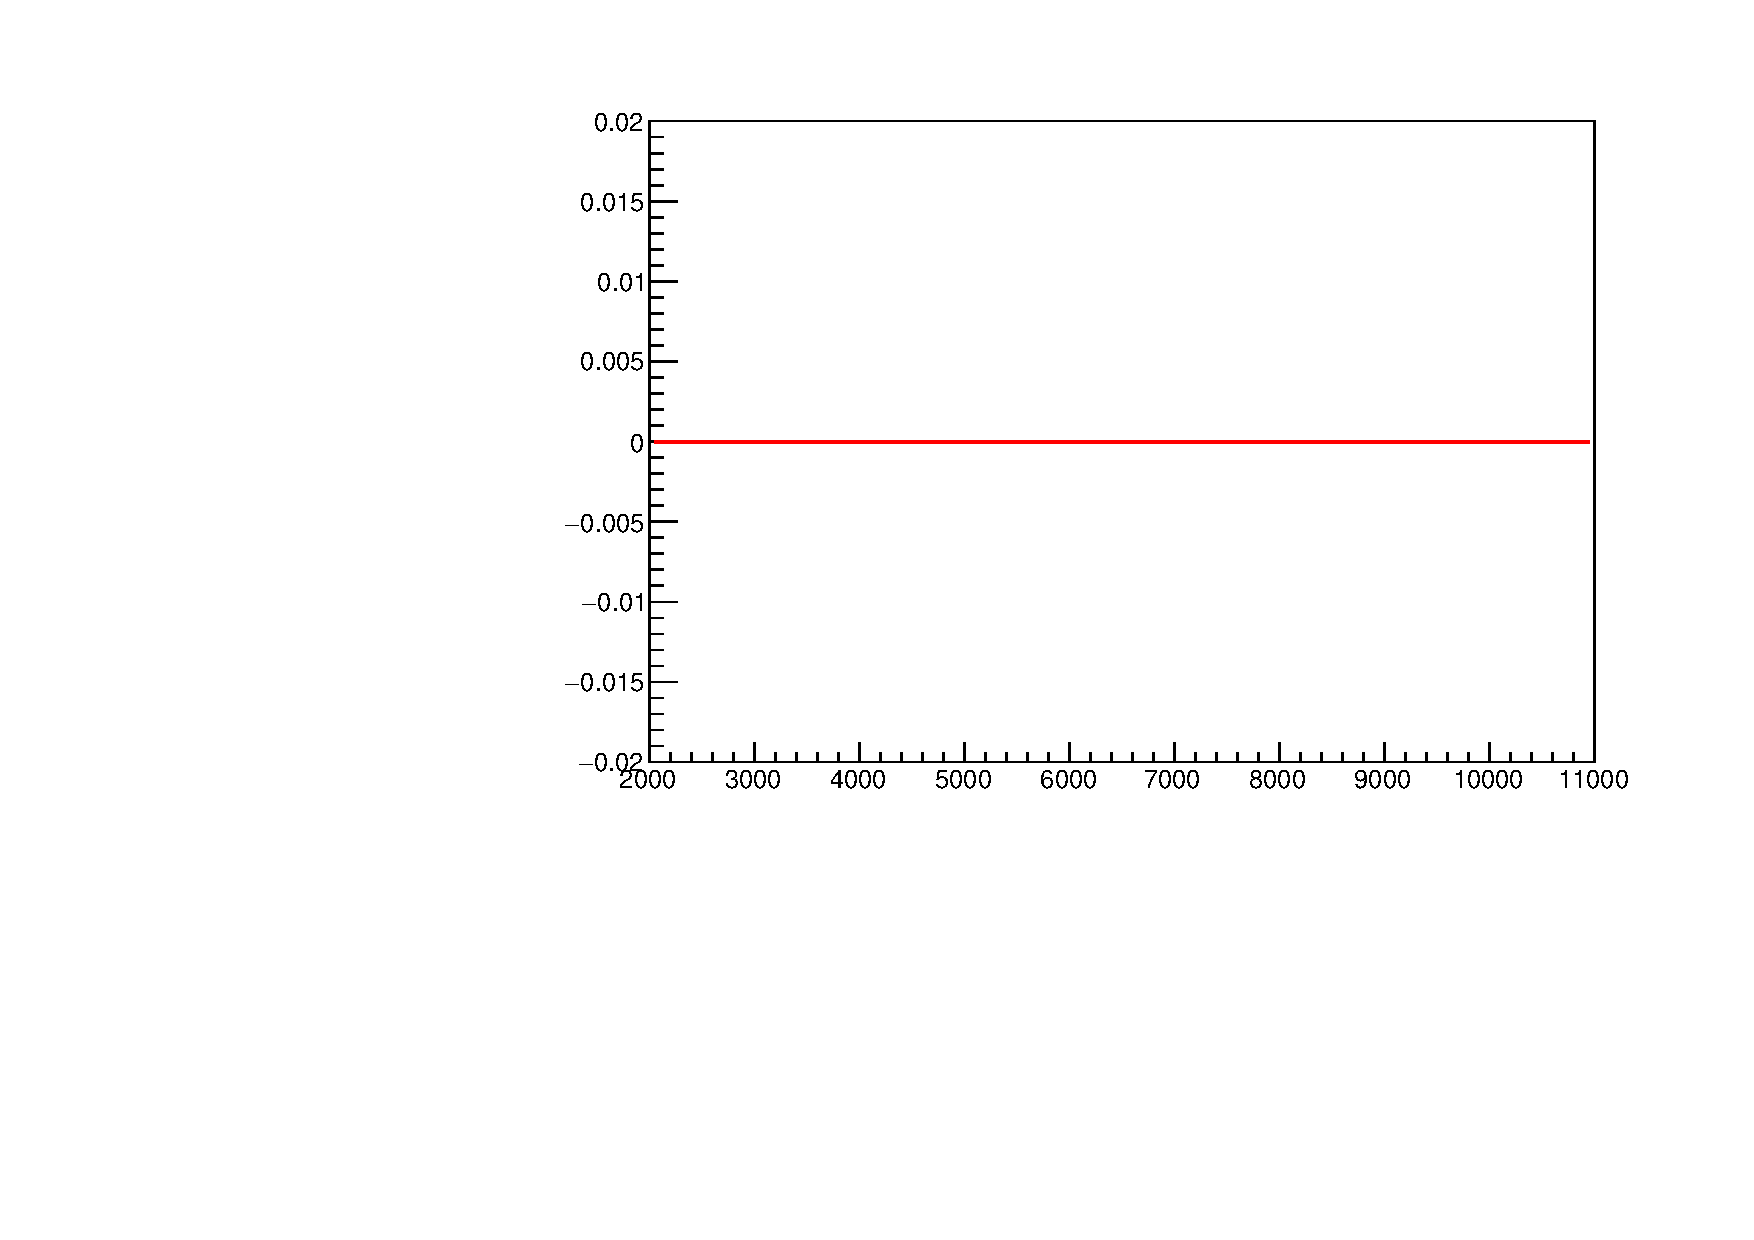
\includegraphics[width=0.9\textwidth]{up_plus_down_pdf/pT_4.pdf}
\end{subfigure}
\begin{subfigure}{0.45\textwidth}
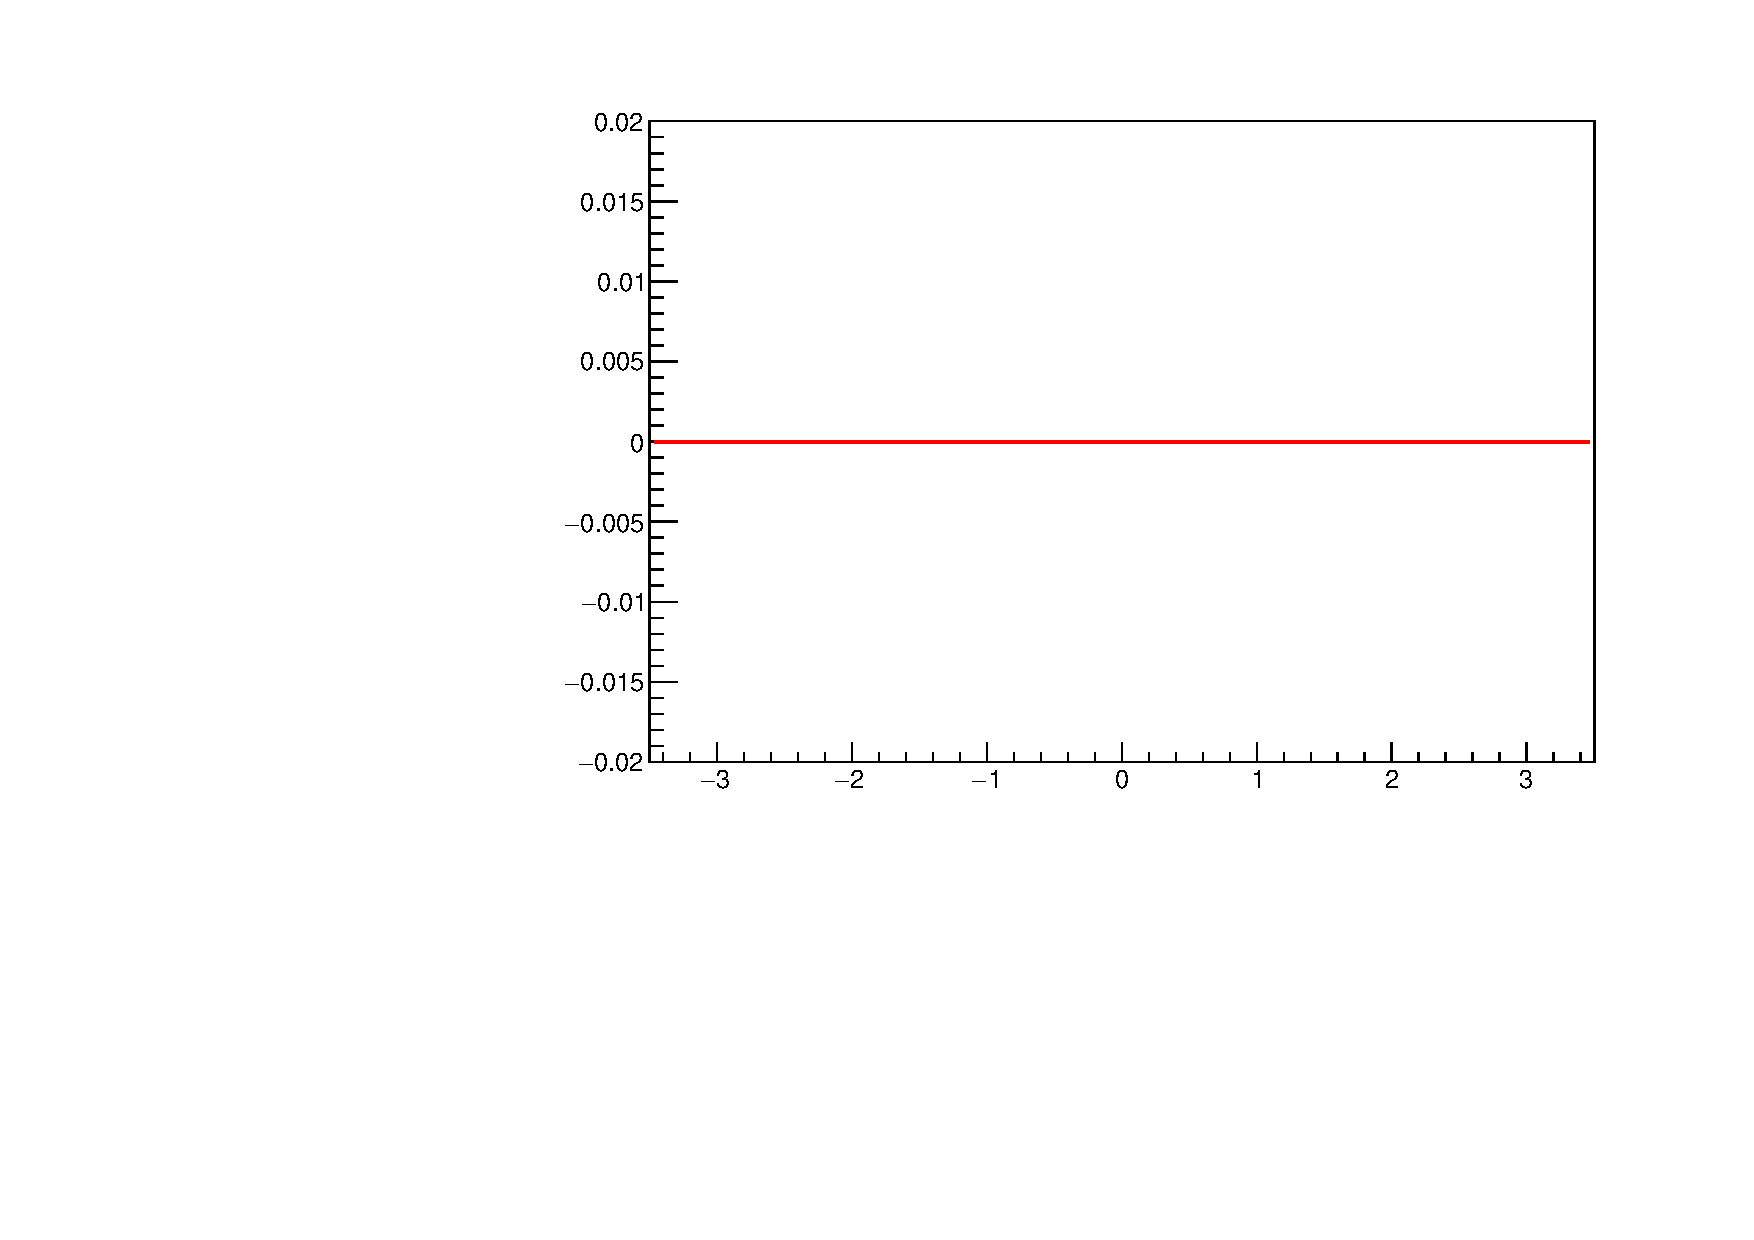
\includegraphics[width=0.9\textwidth]{up_plus_down_pdf/phi_4.pdf}
\end{subfigure}
\begin{subfigure}{0.45\textwidth}
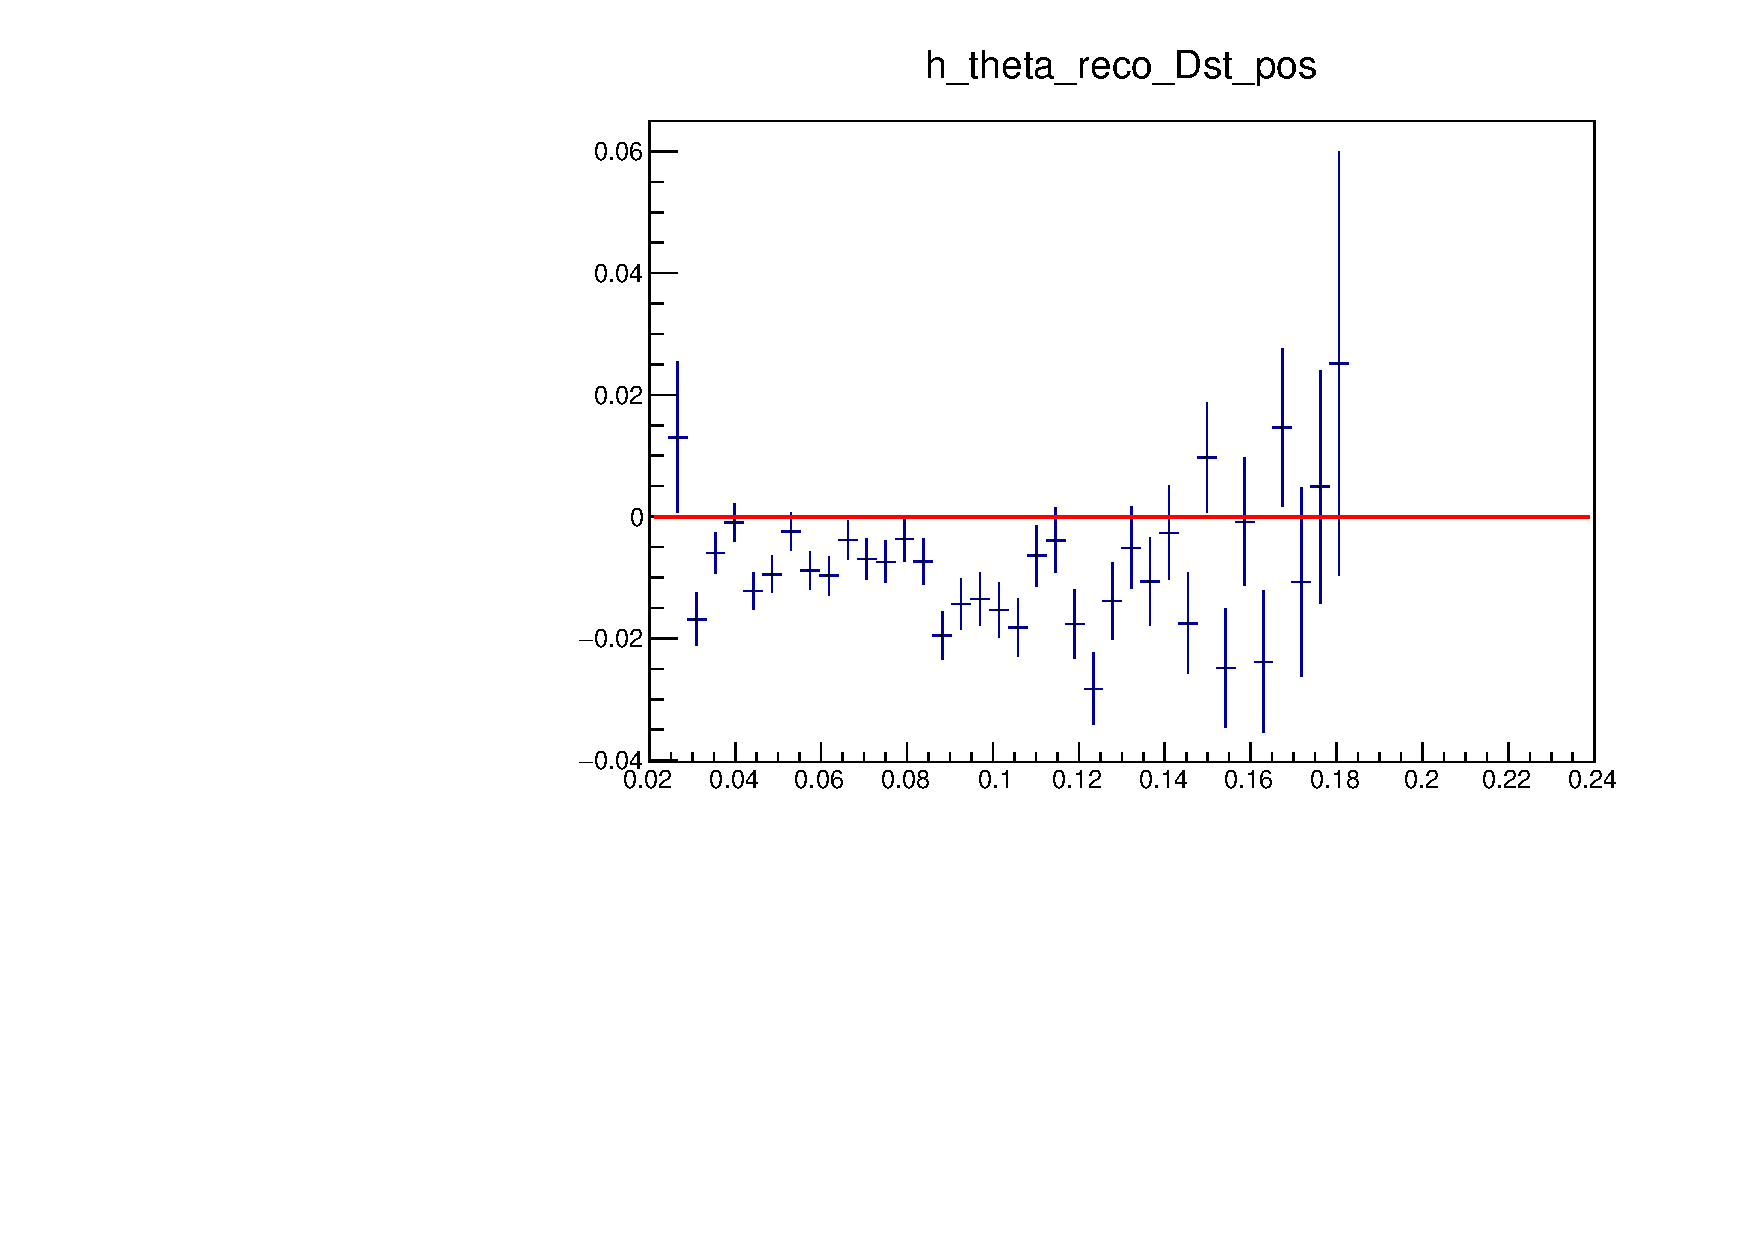
\includegraphics[width=0.9\textwidth]{up_plus_down_pdf/theta_4.pdf}
\end{subfigure}
\begin{subfigure}{0.45\textwidth}
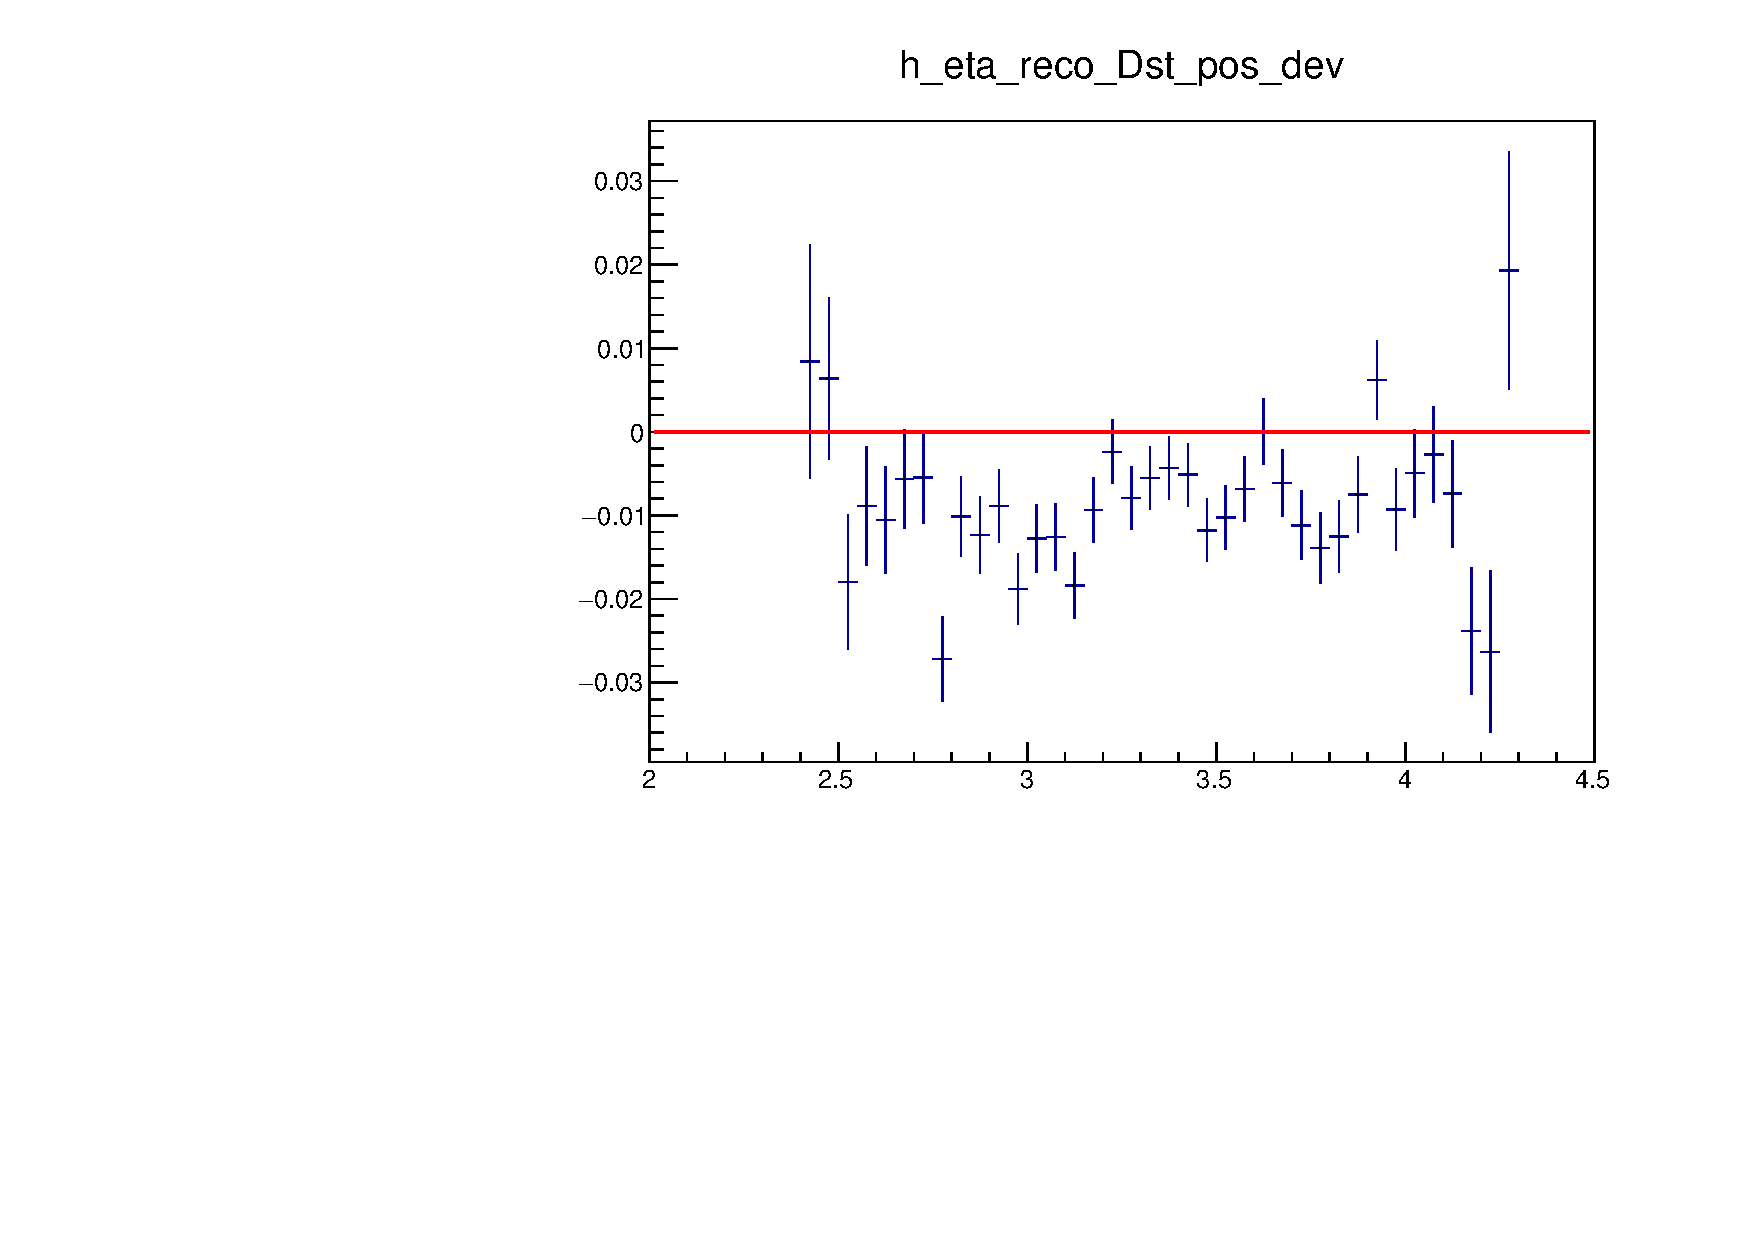
\includegraphics[width=0.9\textwidth]{up_plus_down_pdf/eta_4.pdf}
\end{subfigure}
\end{figure}
\end{frame}
\end{document}


%♥